Esperimenti con i raggi cosmici hanno dimostrato anche la presenza di altre nuove particelle confermate da esperimenti agli accelleratori. Vennero chiamate \textbf{strane}: prodotte con sezione d'urto forte (quindi con una sezione d'urto dell'ordine del $mb$) con un decadimeto con tempi tipici delle interazioni deboli ($10^{-8}-10^{-9}\,s$ che sono i tempi tipici del decadimento del pione che è un processo mediato da interazioni deboli) . Si osserva che venivano sempre prodotte in coppie quindi mi viene in mente che ci sia un nuovo numero quantico conservato: stranezza. Viene conservato nelle interazioni forti mentre violato nelle interazioni deboli. Avevamo visto come la produzione di tutte queste particelle come risonanze potevano essere viste come dei possibili stati legati che possono essere prodotti con quark e antiquark. Consiste nell'introduzione di un nuovo quark: $s$. Questa analisi delle particelle strane porta allo sviluppo della struttura a quark degli adroni. Si passa da $SU(2)$ di spin isotopico a $SU(3)$ di sapore. Le interazioni deboli di questo quark apriranno la strada alla sistematizzazione delle interazioni deboli degli adroni. Possiamo già iniziare a classificare i vari tipi di particelle: un \textbf{adrone} è una particella che interagisce forte, tipicamente composta o da tre quark o da quark e anti-quark (e questo porta gli adroni a dividersi in barioni e mesoni). Mentre le particelle che interagiscono debole o elettromagnetica sono dette \textbf{leptoni} particella + neutrino associato.
\subsection{Particelle strane}
Nell'esposizione di camera a nebbia a raggi cosmici, si misero in evidenza decadimenti di nuove particelle. Le nuove particelle sono pesanti: hanno diversi decadimenti possibili. 

 %IMMAGINE fdf
\begin{figure}[htp!]
  \centering
  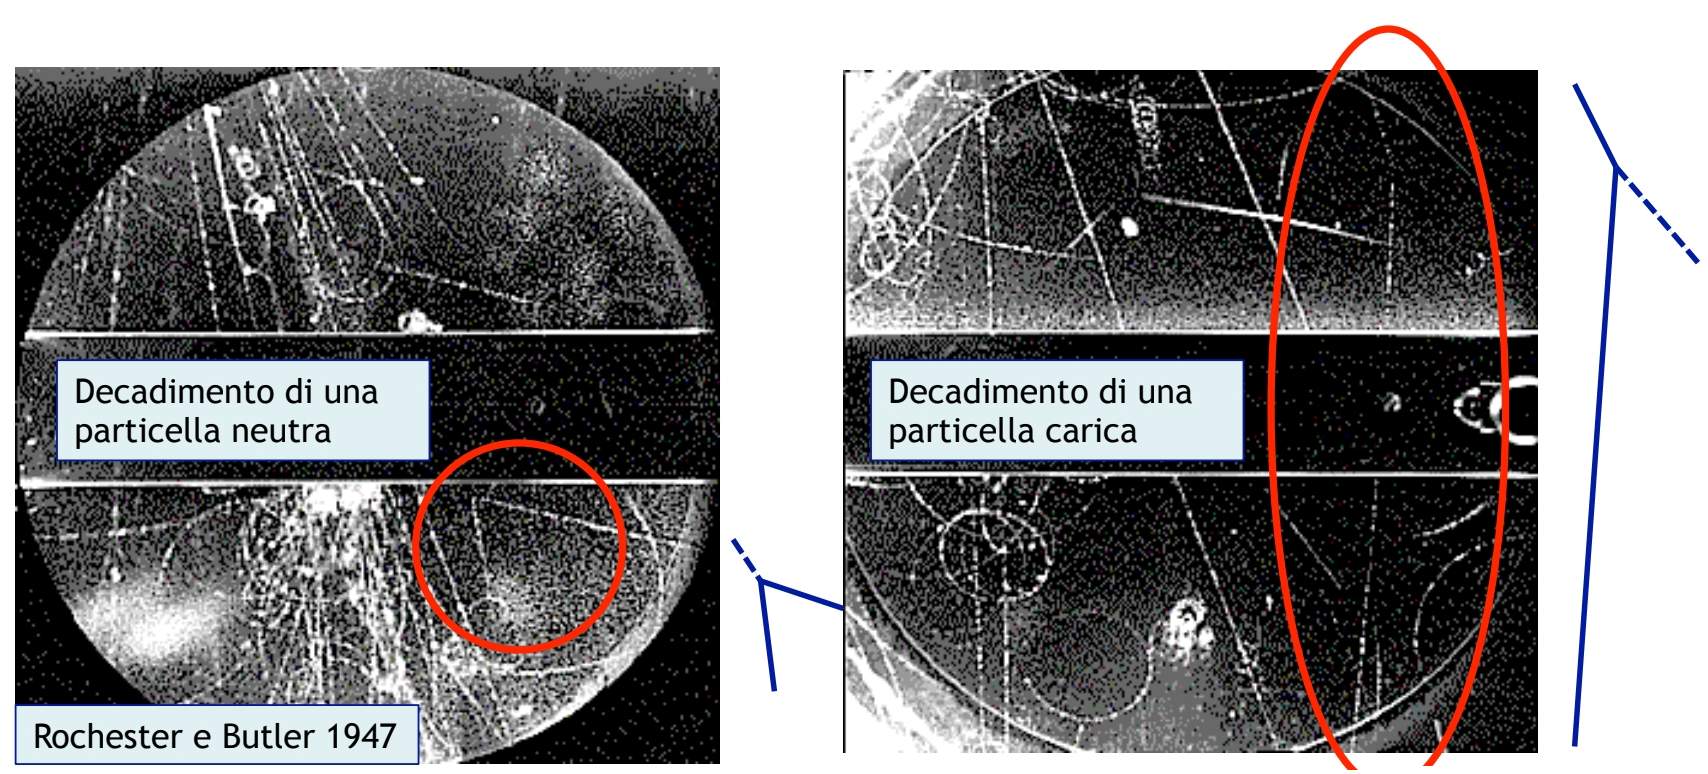
\includegraphics[scale=0.2]{Lezione16/fdf.png} 
\end{figure}
Nella prima immagine a sinistra si può vedere come una particella neutra (invisibile nella camera a nebbia) decade in due particelle di carica opposta. Questo mi sta dicendo che è avvenuta una cerca interazione che ha portato ad una formazione di una particella che poi è decaduta. Nella seconda immagine a destra si può vedere una particella che arriva (ha anche un alto momento perchè la densità di ionizzazione è bassa). La particella è carica ma dopo un po' viene "deviata". Questo rappresenta il fatto che la mia particella è decaduta in una componente carica e in una componente neutra.
In questi esperimenti si poteva ricavare il momento dalla curvatura in campo magnetico ma le informazioni non erano sufficienti per identificare la massa.
Attraverso varie tecniche ed esperimenti si trovano numerose nuove particelle. Le nuove particelle sono pesanti: hanno diversi decadimenti possibili.
In particolare si trovano dei mesoni con stati $J^P=0^-$ (lo spesso del pione) e iperoni (barioni con numero quantico di stranezza diverso da zero) con stati $J^P=1/2^+$ (stesso dei nucleoni). 

Un esempio di mesoni chiamato $K^+$:
\begin{equation*}
    K^+\to \pi^+\pi^+\pi^-\quad K^+\to \pi^+\pi^0 \quad K^+\to \mu^+\nu
\end{equation*}
Quindi si vede (dal terzo decadimento si può vedere che il $K$ può decadere debole esattamente come il pione). Però può decadere anche in due e tre pioni. Calcolando la massa invariante dei due pioni o tre pioni si trova che: $m_{K^+}=493.677\,MeV$. Esiste anche l'analogo neutro:
\begin{equation*}
    K^0\to \pi^+\pi^-
\end{equation*}
Con $m_{K^0}=497.646\,MeV$ che è leggermente superiore. Questa variazione di massa ricorda quando ho variazioni di isospin (tra pione carico e neutro o tra protone e neutrone).

Quando andiamo a vedere iperioni  ne troviamo un bel po':
\begin{equation*}
    \Lambda^0\to p\pi^- \quad \Sigma^+\to p\pi^0 \quad \Sigma^\pm\to \pi^{\pm}\quad \Xi^-\to \Lambda^0\pi^-
\end{equation*}
\begin{equation*}
    m_\Lambda=1115.683\,MeV \qquad m_{\Sigma^+}=1189.37\,MeV
\end{equation*}
\begin{equation*}
    m_{\Sigma^-}=1197.449\,MeV \qquad m_{\Xi^-}=1321.31\,MeV
\end{equation*}
Hanno tutti una massa maggiore dei nucleoni. Hanno vite medie di $10^{-8}-10^{-10}s$: \textbf{decadimenti deboli} anche se sono coinvolti adroni (quindi particelle che interagiscono forte) rimane comunque un decadimento che avviene in interazioni deboli. Questo significa che in questi decadimenti viene rotta una simmetria che non abbiamo ancora introdotto. D'altra parte, dal tasso di produzione si poteva evincere una sezione d'urto in alluminio (involucro della camera a nebbia) dell'ordine del $mb$ e questo al contrario ci suggerisce che la produzione è un \textbf{processo forte}. Quindi abbiamo questa bi-valenza.
\subsection{Numero barionico}
Come possiamo dare un senso a tutte queste nuove particelle strane? Prima di procedere nella nostra discussione sulle particelle strane analizziamo la conservazione del numero barionico. Il decadimento $\beta$ del neutrone: $n\to pe^-\Bar{\nu}$. Questo decadimento è permesso perchè il numero barionico è una quantità conservata (barione nello stato iniziale, barione nello stato finale anche se cambia di sapore). Numero barionico conservato anche se il numero dei singoli protoni e neutroni no. Sorge però una domanda, perchè non esiste il decadimento: $p\to e^+\pi^0$ oppure $e^-p\to \pi^+p^-$ (questo decadimento conserva lo spin, la carica ma non è osservato). Ma nessuno dei due avviene. La vita media del protone ($\tau_p>1.6\times10^{33}$anni) è il risultato degli studi precedenti. L'esperimento consiste nel tenere una grande massa "sotto osservazione". Quindi posso andare a osservare l'attività: $A=\lambda N=N/\tau$. Ma l'attività posso vederla anche come $N_{dec}T$. Quindi $N_{dec}=NT/\tau$. Quindi posso porre un limite a $\tau$ avendo un numero grande di $NT$ osservando per molti anni una quantità grandissima di nucleoni. Ad esempio $1\,cm^3$ di ferro contiene $\rho/AN_AZ=2.2\times10^{24}\,$nuclei$/cm^3$. Un esperimento sensibile richiede pertato: elevata massa ($1000\,ton$) e vasso fondo (caverne, miniere). L'elevato valore di $\tau_p$ suggerisce che il protone sia stabile. Dal momento che il neutrone decade in protone e i decadimenti degli iperoni portano sempre ad un protone si stabilisce che gli iperoni sono barioni e il numero barionico è conservato: in una reazione o decadimento il numero dei barioni è quindi costante (il numero di particelle meno il numero di anti-particelle). Il protone è così stabile perchè per decadere dovrebbe decadere in un altro barione più leggero che non essendoci non può più decadere.
\subsection{Produzione associata}
Questa produzione a particelle la vediamo sempre prodotte a coppie. Questo non lo vediamo mai attraverso i raggi cosmici, per cui queste particelle prodotte le vediamo una alla volta. Dobbiamo fare un esperimento con un flusso di particelle abbastanza grande. Ad esempio il sincrotrone di Brook-heaven:
 %IMMAGINE si
\begin{figure}[htp!]
  \centering
  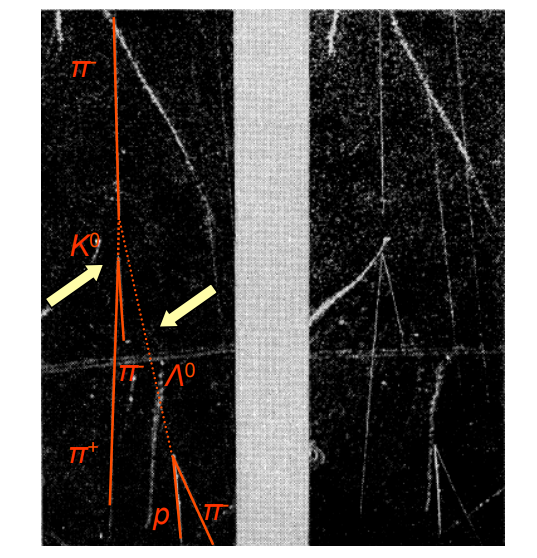
\includegraphics[scale=0.6]{Lezione16/si.png} 
\end{figure}
L'evento fu interpretato come:
\begin{equation*}
    \pi^-\,p\,\to\,\Lambda^0\,K^0
\end{equation*}
Quindi prendo un fascio di $\pi^-$ a $1.5\,GeV$ che interagisce con un protone di un bersaglio e questo pione negativo protone da uno stato neutro formato da due particelle neutre $\Lambda^0$ e $K^0$. La $\Lambda^0$ la vedo perchè dopo un po' decade in uno stato $\Lambda^0\to p\pi^-$. Infatti si vedono due tracce ad intensità di ionizzazione diversa (il protone più le to ionizza molto di più). Il protone va molto più lento quindi la traccia sarà più intensa. Dall'altra parte vedo un'altra particella che decade in maniera simmetrica in due pione: $K^0\to\pi^+\pi^-$. L'importanza di questo evento fu la dimostrazione della produzione associata delle particelle strane. Nello stesso esperimento il gruppo di Fowler osservò anche il processo:
\begin{equation*}
    \pi^-\,p\,\to\,\Sigma^-\,K^+
\end{equation*}
L'osservazione della produzione associata porta all'ipotesi che ci sia una quantità cosnervata: \textbf{la stranezza}
\subsection{Isospin e stranezza: iperoni}
Per spiegare tutte le osservazioni, Gell-Mann e Nishijima proposero di aggiungere un numero quantico additivo, la stranezza che nelle interazioni forti è conservata. Quindi che una particella strana può decadere solo in un'altra particella strana. Se non ci sono altre particelle strane più leggere come se non ci sono barioni più leggeri, la particella strana rimane stabile per le interazioni forti e quindi il decadimento deve avvenire tramite altre interazioni che non conservano la stranezza. Nelle interazioni deboli la stranezza non è conservata ma rispetta una regola ben precisa: $|\Delta S|=1$ nei decadimenti. Avevamo scritto una relazione che lega la carica, il numero barionico e l'isospin di una particella. Ora, includendo la stranezza, la relazione per la carica deve essere modificata:
\begin{equation*}
    Q=\frac{B}{2}+\frac{S}{2}+I_3=\frac{Y}{2}+I_3
\end{equation*}
La $Y=B+S$ viene chiamata iper-carica. Vale anche in ambito più ampio. In questo modello tutti i barioni visti prodotti all'interno della camera a bolle li possiamo classificare in base ai numeri quantici di carica, numero barionico (sono tutti barioni quindi $B=1$), la carica. La $\Xi$ è in due stati di carica che decade in una particella strana che decade in un'altra particella strana o in $\Sigma$ o in $\Lambda$ e dopo decadono in $n$ o $p$. Risalendo questa catena si deduce che hanno stranezza $S=-2$. Con questa cosa abbiamo una generalizzazione di questa legge. 
 %IMMAGINE t
\begin{figure}[htp!]
  \centering
  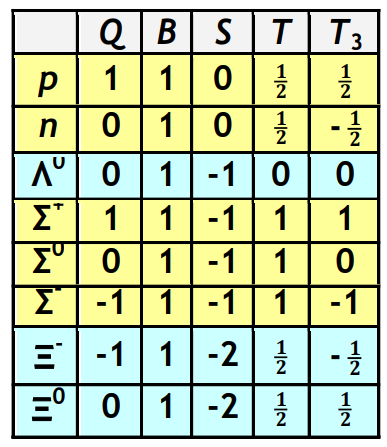
\includegraphics[scale=0.6]{Lezione16/t.png} 
\end{figure}
\subsection{Isospin e stranezza: mesoni}
Innanzitutto consideriamo la reazione:
\begin{equation*}
    \pi^-\,p\,\to\,\Lambda^0\,K^0
\end{equation*}
che per quanto riguarda i numeri di stranezza:
\begin{equation*}
    0\,0\,\xrightarrow[]{S}\,-1\,1
\end{equation*}
Assumento che nella interazione forte la stanezza sia conservata dobbiamo concludere che il mesone $K^0$ abbia $S=+1$. Per quanto riguarda l'isospin assumiamo che esso sia conservato nella reazione di produzione, assumento che sia una reazione forte dalla sezione d'urto abbiamo che anche l'isospin si deve conservare:
\begin{equation*}
    \pi^-\,p\,\to\,\Lambda^0\,K^0
\end{equation*}
che per quanto riguarda il numero di isospin:
\begin{equation*}
    1\,\frac{1}{2}\,\xrightarrow[]{T}\,0\,?
\end{equation*}
Quindi sicuramente deve essere semintero, assumiamo che il $K^0$ abbia isospin $T=1/2$. La formula per la carica applicata al $K^0$ implica che esso è il menbro $T_3=-1/2$ di un doppietto. Il membro $T_3=1/2$ deve avere carica $+1$ ed è pertanto il mesone $K^+$. IL mesone $K^-$ è l'antiparticella del $K^+$ anch'esso deve avere isospin $I=1/2$ deve esserci anche un parner neutro: $\Bar{K^0}$. Le particelle $K^0$ e $\Bar{K^0}$ sono distinti infatti hanno stranezza opposta. Infatti per quanto riguarda il neutrone riuscivamo a distinguere neutrone e anti-neutrone dal numero barionico (risultava ovviamenteo opposto). In questo caso il numero quantico che ci permette di distinguere le due particelle è la stranezza. In definitiva i numeri quantici dei mesoni sono:
 %IMMAGINE i
\begin{figure}[htp!]
  \centering
  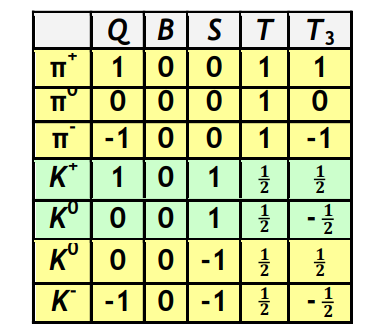
\includegraphics[scale=0.6]{Lezione16/i.png} 
\end{figure}
\subsection{Decadimento delle particelle strane}
Le particelle strane decadono tramite interazione debole che violano la conservazione della stranezza. Le prime particelle strane studiate sono anche le più leggere. Possono decadere soltato in particelle "normali" con $S=0$. La violazione della stranezza proibisce che l'interazione sia forte. Infatti i seguenti decadimenti che soddisfano e sarebbero permessi dalla conservazione della stranezza sono proibiti dalla conservazione dell'energia:
\begin{equation*}
    \Lambda\to N\Bar{K} \quad \Sigma\to N\Bar{K} \quad \Xi\to \Lambda\Bar{K} \quad \Xi\to \Sigma\Bar{K} \quad \Sigma \to \Lambda\pi
\end{equation*}
Il decadimento 
\begin{equation*}
    \Sigma^0\to \Lambda^0\gamma
\end{equation*}
Questo sarebbe possibile sia in termini energetici che per quanto riguarda la conservazione della stranezza ma non si conserva lo spin isotopico. Lo spin isotopico può essere violato nelle interazioni elettromagnetiche. Quindi nelle interazioni elettromagnetiche siamo in una situazioni strane perchè viene conservata la stranezza ma non lo spin isotopico.

Ricapitolando abbiamo introdotto un nuovo numero quantico la stranezza che viene conservato nelle interazioni forti ed elettromagnetiche. Nelle interazioni deboli no e questo giustificava le particelle strane. Quindi particelle prodotte in interazioni forti ma poi i decadimenti di una singola particella strana visto che richiedono masse inferiori (richiedono di passare a particelle non strane) attraverso interazioni che violano questa legge di conservazione. Andiamo a vedere come questra stranezza si traduce poi in un'ipotesi sui costituenti della materia.
\subsection{Interpretazione nel modello a quark}
Avevamo già introdotto questo modello facendo vedere che le varie risonanze le potevamo vedere come diversi stati legati di due sole particelle fondamentali quark-up e quark-down.
Il modello a quark si può estendere con l'aggiunta di un nuovo quark: $s$ con stranezza $S=-1$, $B=1/3$, $Y=-2/3$, $I=I_3=0\Rightarrow Q=-1/3$. La massa: $m_s\sim m_K-m_\pi=360\,MeV$. Gli adroni sono stati legati dei $3$ quark $u$, $d$, $s$. Come esempio notiamo la composizione dei seguenti adroni: i barioni costituiti da $3$ quark e i mesoni costituiti da quark e anti-quark.
\begin{equation*}
    p=(uud)\qquad \Lambda=(uds) \qquad \pi^-=(\Bar{u}d) \qquad K^0=(d\Bar{s})
\end{equation*}
Veniamo alla reazione $\pi^- p\to \Lambda^0K^0$ lo possiamo vedere come un processo tale per cui i quark $u$ e $\Bar{u}$ si annichilano tramite interazione forte (gluone) e producono successivamente quarks $s$ e $\Bar{s}$
 %IMMAGINE h
\begin{figure}[htp!]
  \centering
  
\includegraphics[scale=0.5]{Lezione16/h.png} 
\end{figure}
Per il decadimento $\Lambda^0\to\pi^- p$ in questo caso il quark $s$ si trasforma in $u$ tramite interazione debole (emissione $W$)
%IMMAGINE h1
\begin{figure}[htp!]
  \centering
  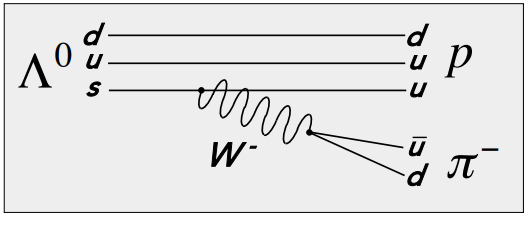
\includegraphics[scale=0.5]{Lezione16/h1.png} 
\end{figure}
\subsection{SU(3) di sapore}
Reiteriamo l'idea che le interazioni forti sono indipendenti dalla carica dei quark (sia elettrica che di ipercarica). Invarianza rispetto a rotazione nello spazio di tre stati $|u\rangle$, $|d\rangle$ e $|s\rangle$. Si dice che le interazioni forti non dipendono dal tipo di quark quindi sono indipendenti dal sapore dei quark. Noi possiamo mettere i quark in un diagramma in cui nelle ordinate c'è l'iper-carica e nelle ascisse lo spin isotopico:
%IMMAGINE tt
\begin{figure}[htp!]
  \centering
  
\includegraphics[scale=0.6]{Lezione16/tt.png} 
\end{figure}
Dal momento in cui abbiamo 3 quark stiamo andando, al posto di essere bidimensionale nel caso della simmetria dello spin isotopico, in uno spazio tridimensionale al gruppo $SU(3)$ matrici unitarie nello spazio a tre dimensioni. La massa delle particelle strane $>>$ nelle particelle ordinarie. Qui abbiamo una cosa molto diversa nello spin isotopico, infatti avevamo visto che le differenze di massa erano nell'ordine di qualche $MeV$ al fronte di centinaia o migliaia di $MeV$ delle stesse particelle e questa asimmetria potevamo attribuirla all'effetto delle interazioni elettromagnetiche era una piccola correzione. Nel caso di particelle strane che hanno una massa maggiore, la simmetria è meno buona di quella di isospin.
\subsection{Gruppi SU(N)}
Per definizione, una matrice $n\times n$ del gruppo $U(N)$ che soddisfa la relazione di unitarietà: $UU^\dagger=I$ e $S$ sta per speciale perchè sono matrici con determinante uguale a $1$. L'equazione precedente implica $n\times n$ relazione fra gli $n\times n$ elementi di matrice. Pertanto dei $2\times n \times n$ parametri reali ho solo $2\times n \times n-n\times n=n\times n$ sono indipendenti. La richiesta poi che il determinate sia $1$ riduca di un'altra unità questo numero. Peranto i paramentri indipendenti dei $2$ gruppi più importanti per la fisica delle particelle sono $SU(2)$ con 3 parametri reali (i tre angoli di rotazione) e $SU(3)$ con 8 parametri reali. Venendo alle rappresentazioni: una rappresentazione è un omomorfismo di un gruppo con un gruppo di matrici definite su uno spazio vettoriale di dimensione $n$. I fisici spesso chiamano rappresentazione i vettori dello spazio vettoriale (quindi matrici dello spazio vettoriale). Quando noi parliamo di doppietto e tripletto noi chiamiamo doppietto come possibile rappresentazione del gruppo $SU(2)$ il tripletto invece come possibile rappresentazione del gruppo $SU(2)$ con tutte le varie combinazioni. 

Tutti i gruppi hanno una rappresentazione banale di dimensione 1 che corrisponde all'elemento 1. La dimensione della rappresentazione di dimensione più piccola successiva dipende dal gruppo. $SU(2)$ è realizzata su uno spazio vettoriale di dimensione $2$ che ad esempio è proprio lo spin $1/2$. Coincide con la rappresentazione coniugata delle matrici $U^*$ tra particelle e antiparticelle. Una sola rappresentazione: 2

Per $SU(3)$ è realizzata su uno spazio vettoriale di 3 dimensioni. Non coincide con la rappresentazione coinugata delle matrici $U^*$. Due rappresentazioni: $3$ e $3^*$ dove la prima regola le leggi di trasformazioni dei quark mentre la seconda degli anti-quark.
\subsection{La rappresentazione 3 di SU(3)}
Le $8$ matrici della rappresentazione $3$ (matrici di Gell-Mann) sono:
\begin{equation*}
    {\displaystyle \lambda _{1}:={\begin{pmatrix}0&1&0\\1&0&0\\0&0&0\end{pmatrix}}~,\quad \lambda _{2}:={\begin{pmatrix}0&-i&0\\i&0&0\\0&0&0\end{pmatrix}}~,\quad \lambda _{3}:={\begin{pmatrix}1&0&0\\0&-1&0\\0&0&0\end{pmatrix}}~,\quad \lambda _{4}:={\begin{pmatrix}0&0&1\\0&0&0\\1&0&0\end{pmatrix}}~,}
\end{equation*}
\begin{equation*}
    {\displaystyle \lambda _{5}:={\begin{pmatrix}0&0&-i\\0&0&0\\i&0&0\end{pmatrix}}~,\quad \lambda _{6}:={\begin{pmatrix}0&0&0\\0&0&1\\0&1&0\end{pmatrix}}~,\quad \lambda _{7}:={\begin{pmatrix}0&0&0\\0&0&-i\\0&i&0\end{pmatrix}}~,\quad \lambda _{8}:={\frac {1}{\sqrt {3}}}{\begin{pmatrix}1&0&0\\0&1&0\\0&0&-2\end{pmatrix}}~.}
\end{equation*}
Dove le prime tre ci ricordano che questo $SU(3)$ lo possiamo vedere come un gruppo di simmetria che continene la simmetria di spin isotopico. Sono le matrice di $SU(2)$ in una dimensione più grandi perchè oltre al wuark up e down bisogna tener conto del quark strano. Quindi come le prime $3$ ci danno le rotazioni dello spazio dei quark up e down le matrici $4$ e $5$ tengono conto delle rotazioni tra quark up e quark s. Oppure rotazioni tra quark d e quark s per le matrici $6$ e $7$. Come ottavo elemento ottengo la terza matrice che manca delle rotazioni tra d s o u s. La generica rotazione:
\begin{equation*}
    U=\text{exp}\left[i\sum_{n=1}^8 \alpha_n\lambda_n\right]
\end{equation*}
Le regole di commutazione:
\begin{equation*}
    [\lambda_i,\lambda_j]=2if_{ijk}\lambda_k
\end{equation*}
Dove il coefficiente $f_{ijk}$ è tabulato. Si definiscono gli operatori $T_3$ e $Y$:
\begin{equation*}
    Y=\frac{1}{\sqrt{3}}\lambda_8 \qquad T_3=\frac{1}{2}\lambda_3
\end{equation*}
Comportamento sulla base:
\begin{equation*}
    |u\rangle=\left(\begin{array}{l}1 \\ 0 \\ 0\end{array}\right)\quad|d\rangle=\left(\begin{array}{l}0 \\ 1 \\ 0\end{array}\right)\quad|s\rangle=\left(\begin{array}{l}0 \\ 0 \\ 1\end{array}\right)
\end{equation*}
infatti:
\begin{equation*}
    T_3|u\rangle=\frac{1}{2}|u\rangle \qquad Y|u\rangle=\frac{1}{3}|u\rangle
\end{equation*}
\begin{equation*}
    T_3|d\rangle=-\frac{1}{2}|d\rangle \qquad Y|d\rangle=\frac{1}{3}|d\rangle
\end{equation*}
\begin{equation*}
    T_3|s\rangle=0|s\rangle \qquad Y|s\rangle=-\frac{2}{3}|s\rangle
\end{equation*}
%IMMAGINE po
\begin{figure}[htp!]
  \centering
  
\includegraphics[scale=0.6]{Lezione16/po.png} 
\end{figure}
\subsection{Operatori di SU(3)}
Abbiamo visto il comportamento degli stati per gli operatori $T_3$ e $Y$. Definiamo gli operatori:
\begin{equation*}
    F_i=\frac{1}{2}\lambda_i
\end{equation*}
Gli operatori $F_1$, $F_2$, $F_3$$\equiv T_3$ ed hanno le stesse regole di commutazione dell'isospin:
\begin{equation*}
    [F_i,F_j]=if_{ijk}F_k
\end{equation*}
Dove $f_{ijk}$ è totalmente antisimmetrico e $f_{123}=1$ e coincide pertanto con $\varepsilon_{123}$. Infatti riconosciamo le matrici di pauli nelle prime tre matrici. Definiamo pertanto gli operatori di innalzamento e di abbassamento:
\begin{equation*}
    T_{\pm}=F_1\pm iF_2 \quad V_{\pm}=F_4\pm iF_5 \quad V_3=\frac{1}{2}(F_3+\sqrt{3}F_8) \quad U_{\pm}=F_6\pm iF_7 \quad u_3=\frac{1}{2}(-F_3+\sqrt{3}F_8)
\end{equation*}
Le regole di commutazione fra questi nuovi operatori sono facilmente derivabili.
\subsection{La rappresentazione 3coniugato di SU(3)}
Analogamente si può studiare la rappresentazione coniugata in cui generatori sono:
\begin{equation*}
    \lambda_n\to-\lambda_n^*
\end{equation*}
Definiamo nuovamente:
\begin{equation*}
    Y=-\frac{1}{\sqrt{3}}\lambda_8^*\qquad T_3=-\frac{1}{2}\lambda_3^*
\end{equation*}
Studiamo infine l'effetto dei generatori diagonali sulla base:
\begin{equation*}
    |\Bar{u}\rangle=\left(\begin{array}{l}1 \\ 0 \\ 0\end{array}\right)\quad|\Bar{d}\rangle=\left(\begin{array}{l}0 \\ 1 \\ 0\end{array}\right)\quad|\Bar{s}\rangle=\left(\begin{array}{l}0 \\ 0 \\ 1\end{array}\right)
\end{equation*}
Abbiamo:
\begin{equation*}
    T_3|\Bar{u}\rangle=-\frac{1}{2}|\Bar{u}\rangle \qquad Y|\Bar{u}\rangle=-\frac{1}{3}|\Bar{u}\rangle
\end{equation*}
\begin{equation*}
    T_3|\Bar{d}\rangle=\frac{1}{2}|\Bar{d}\rangle \qquad Y|d\rangle=-\frac{1}{3}|\Bar{d}\rangle
\end{equation*}
\begin{equation*}
    T_3|\Bar{s}\rangle=0|\Bar{s}\rangle \qquad Y|\Bar{s}\rangle=\frac{2}{3}|\Bar{s}\rangle
\end{equation*}
%IMMAGINE po1
\begin{figure}[htp!]
  \centering
  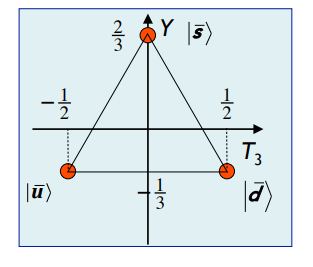
\includegraphics[scale=0.6]{Lezione16/po1.png} 
\end{figure}
\subsection{Ottupletto mesonico}
Nel modello a quark i mesoni sono uno stato legato di un quark e di un antiquark. Per i 3 sapori esistono 9 possibili combinazioni di quark e antiquark che possiamo formare.
%IMMAGINE ott
\begin{figure}[htp!]
  \centering
  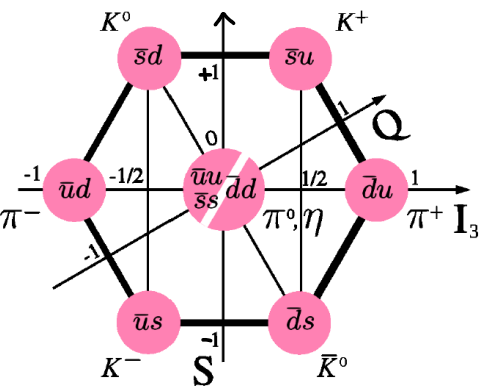
\includegraphics[scale=0.6]{Lezione16/ott.png}
  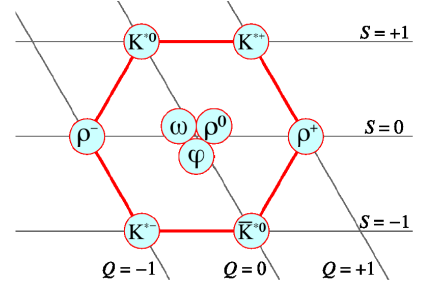
\includegraphics[scale=0.6]{Lezione16/po2.png}
\end{figure}
Gli stati con $I_3=Y=0$ sono una combinazione lineare che hanno i numeri quantici corrispondenti a stati fisici, in particolare se noi applichiamo la trasformazione $T_+$ al $\pi^-$ o applichiamo $T_-$ al $\pi^+$ otteniamo:
\begin{equation*}
    \frac{1}{\sqrt{2}}=\left(u\Bar{u}-d\Bar{d}\right)=\pi^0 \qquad T=1 \quad T_3=0
\end{equation*}
\begin{equation*}
    \frac{1}{\sqrt{6}}=\left(u\Bar{u}+d\Bar{d}-2s\Bar{s}\right)=\eta \qquad T=0 \quad T_3=0
\end{equation*}
\begin{equation*}
    \frac{1}{\sqrt{3}}=\left(u\Bar{u}+d\Bar{d}+s\Bar{s}\right)=\eta' \qquad T=0 \quad T_3=0
\end{equation*}
Quindi $\eta'$ vale la rappresentazione di singoletto in quanto quando applico una rotazione non cambia. Singoletto di $SU(3)$. Mentre tutte le altre sono oggetti che possono essere trasformati uno in un altro attraverso trasformazioni di $SU(3)$. Se $SU(3)$ fosse una simmetria esatta avrei di fatto 8 stati degeneri che sono quelli dell'ottupletto e un altro autostato che potrebbe avere un autovalore di massa diverso che è il singoletto. Ora siccome la simmetria di $SU(3)$ e rotta dal fatto che la massa di $s$ è molto maggiore rispetto alla massa degli altri quark, questo mi può portare ad avere autostati che sono leggermente diversi da questa suddivisione.
\subsection{Classificazione dei barioni}
Anche nel caso dei barioni si possono classificare gli stati possibili in termini di $I_3$ ed ipercarica: $Y=(B+S)/2$. Gli stati fondamentali corrispondono ad un ottetto ed un decupletto:
%IMMAGINE gh
\begin{figure}[htp!]
  \centering
  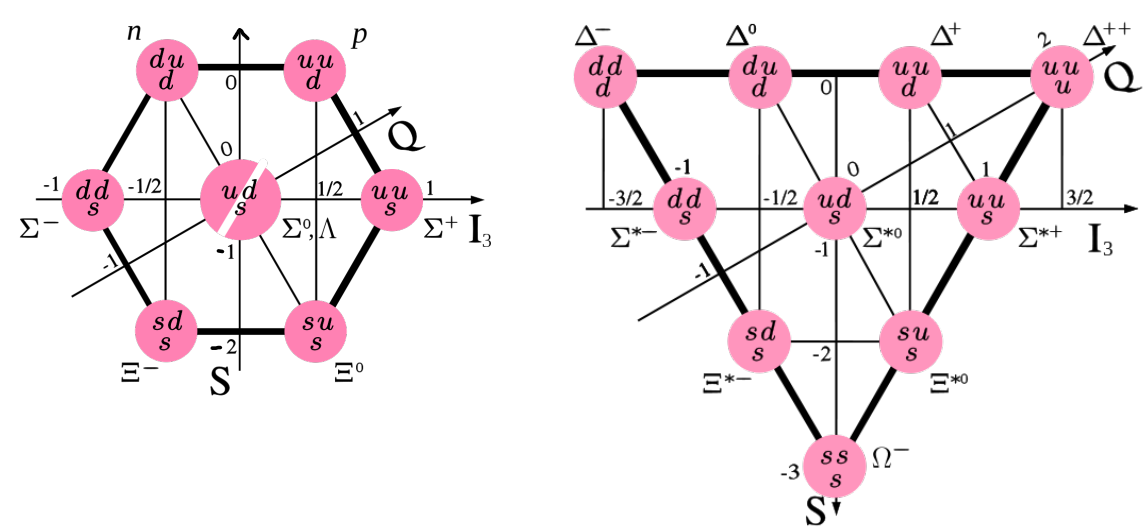
\includegraphics[scale=0.45]{Lezione16/gh.png} 
\end{figure}
Con 3 quark abbiamo 3 possibili sapori, e quindi ci aspettiamo $3\times3\times3=27$ diversi stati ma qui ne vedo solamente $18$. Questo è perchè in questo approccio di $SU(3)$ abbiamo che gli oggetti fondamentali sono i quark che sono dei fermioni. $SU(3)$ di sapore come per $SU(2)$ di isospin dice: particelle con lo stesso multipletto di isospin sono la stessa particella semplicemente con un numero quantico interno diverso. Quello che succede qui è che ho un'unica particella il quark che può esistere in tre diversi stati, la sua funzione d'onda essendo un fermione deve essere anti-simmetrica e quello che scopriremo è che riusciamo a creare funzioni d'onda completamente antisimmetriche solamente per l'ottetto e il decupletto. L'altro decupletto più un singoletto questi non riesco a creare una funzione d'onda antisimmetrica quindi non possono esistere fisicamente.
\subsection{La scoperta del barione omega}
Un significativo successo del modello a quark fu la predizione dell'esistenza di uno stato $(sss)$:
\begin{equation*}
    B=1, \,I=0,\,S=-3,\,Q=-1
\end{equation*}
Scoperto nel 1964 in un esperimento in camera a bolle:
%IMMAGINE lo
\begin{figure}[htp!]
  \centering
  
\includegraphics[scale=0.5]{Lezione16/lo.png} 
\end{figure}
Per produrre tre quark strani mi servirebbe molta energia quindi per comodità anzichè fare un fascio di pioni uso i $K^-$ così lo porto già in uno stato iniziale con un quark strano e ne devo solo produrre due in più.
\subsection{Decadimento dei mesoni K}
Applichiamo lo stesso approccio del decadimento $\beta$ ai mesoni $K$:
\begin{equation*}
    \lambda=\frac{G_F^2|M_{fi}|^2(m_ec^2)^5}{2\pi^3\hbar}f(Z,Q)
\end{equation*}
Nel caso $Q>>m_e$, si ha che:
\begin{equation*}
    (m_ec^2)^5f(Z,Q)\approx\frac{Q^5}{30}
\end{equation*}
Quello che avevamo visto nei decadimenti $\beta$ è che i decadimenti particolari in cui andavo da uno stato $0^+$ ad uno stato $0^+$ l'elemento di matrice era $\sqrt{2}$ (usando la simmetria di radice isotopica).
Nel caso del decadimento:
\begin{equation*}
    \Bar{K}^0\,\to\,\pi^+\,+\,e^-\,+\,\Bar{\nu}_e
\end{equation*}
Questo decadimento sembra molto un decadimento $\beta$ speciale in quanto lo stato inziale ha spin zero, lo stato finale è pure spin zero e ho la produzione di una coppia elettrone antineutrino. Posso stimare l'elemento di matrice osservando che la trasformazione da $ \Bar{K^0}$ a $\pi^+$ è l'effetto dell'operatore $V_+$.
\begin{equation*}
    M_{fi}\approx\langle\pi^+|V_+|\Bar{K}^0\rangle=1
\end{equation*}
Questa è un'approssimazione peggiore di quella per i decadimenti super-permessi. Quindi non potrei trascurare i fattori di forma $f(q^2)$. Otteniamo:
\begin{equation*}
    \Gamma\left(\Bar{K}^0\to\pi^++e^-+\Bar{\nu}_e\right)=\frac{G_s^2(m_K-m_\pi)^5}{60\pi^2}
\end{equation*}
\begin{align*}
     m_K-m_\pi=497.6-139.6 \mathrm{MeV} \\  \tau_{\mathrm{K}_{\mathrm{L}}^0}=(5.116 \pm 0.021) \times 10^{-8} \mathrm{~s} \\  B R\left(K_L^0 \rightarrow \pi^{+} e^{-} \bar{v}_e\right)=(40.55 \pm 0.11) \%
\end{align*}
Ricordando che dalla vita media sappiamo che la larghezza totale è $\hbar/\tau$. La larghezza in uno specifico canale è data dalla larghezza totale moltiplicata per il $BR$ di quel canale.
Possiamo mettere insieme questi valori e ottenere $G_s=0.13\times10^{-5}\,GeV^{-2}$. Che è molto minore di $G_F\approx 1.16\,\times10^{-5}\,GeV^{-2}$ cioè la costante nei decadimenti $\beta$ o quelli del muone. Questo è un risultato che ha fatto riflettere. Prima ho visto che le interazioni deboli avevano un comportamento universale (descritti dalla stessa costante). Ma smette di funzionare quando vado a vedere le particelle strane. Questo disaccordo è stato un punto focale per capire come trattare le interazioni deboli. 
\subsection{L'angolo di Cabibbo}
Facendo un trattamento accurato dei fattori di forma nei decadimenti delle particelle strane, si ottiene:
\begin{equation*}
    \frac{G_s}{G_F}=0.2252\pm0.0009
\end{equation*}
Dai decadimenti $\beta$ abbiamo visto che $G_\beta/G_F$ è vicino ad uno ma non è esattamente uno con tante deviazionistandard. Se confrontiamo questi tre valori notiamo che:
\begin{equation*}
    G_\beta^2+G_s^2=G_F^2
\end{equation*}
Che può anche venire riscritta introducendo un angolo $\theta_C$ (angolo di Cabibbo):
\begin{equation*}
    G_\beta^2\cos^2{\theta_C}+G_s^2\sin^2{\theta_C}=G_F^2
\end{equation*}
Ciò permette di conservare l'universalità delle interazioni deboli assumnedo che il quark che partecipa alle interazioni devoli sia:
\begin{equation*}
    u\leftrightarrow d'=\cos{\theta_C}d+\sin{\theta_C}s
\end{equation*}
Mentre nel decadimento del muone ho un solo parthner con cui può fare interazione e cioè il neutrino. Questa interazione ha quindi la costante di accoppiamento massima (che è quella di fermi). Invece il quark u si trova di fatto ad avere due quark che hanno la carica giusta per fare interazione debole che sono lo strano e il down. Il quark con cui lui si accoppia non è solo uno dei due ma anche una combinazione lineare dei due. Sostanzialmente quando u vorrà interagire con d avrà un peso il coseno mentre al contrario quando u vorrà interagire con s avrà un peso il seno. Questo giustifica il fatto che $G_\beta/G_F$ e $G_s/G_F$ siano due numeri tale per cui se li sommo in quadratura mi danno 1. Quando qualcuno guarda questa teoria pensa no vabbe che schifo anche Cabibbo stesso diceva che le cose facevano un po' schifo. Si vuole qualcosa di più simmetrico. Bisogna introdurre un quarto quark.
\subsection{Il quarto quark}
Le teoria di Cabibbo presenta una forte asimmetria tra il quark u da una parte e la combinazione lineare di d ed s dall'altra. Ciò portò a supporre l'esistenza di un quarto quark, il charm (c). Ha la stessa carica del quark u. L'introduzione del nuovo quark necessita di un nuovo numero quantico di charm, $C$: conservato nelle interazioni forti ed elettromagnetiche ma violato nelle deboli:
\begin{equation*}
    Y=B+S+C \qquad Q(c)=+\frac{2}{3}
\end{equation*}
Probabilità di transizione nei decadimenti deboli, mediata da una matrice mescolamento:
\begin{equation*}
    \left(\begin{array}{ll}u & c\end{array}\right)\left(\begin{array}{cc}\cos \theta_c & \sin \theta_c \\ -\sin \theta_c & \cos \theta_c\end{array}\right)\left(\begin{array}{c}d \\ s\end{array}\right)
\end{equation*}
Cioè il quark u può trasformarsi in d o s con pesi visti prima. Mentre il quark c si può trasfromare in d o s con pesi diversi. Questo quark poi è stato effettivamente scoperto nel 1974 con $m_c\sim1.6\,GeV$. Il modo in cui è stato scoperto è simile alle situazioni di risonanza:
%IMMAGINE io
\begin{figure}[htp!]
  \centering
  
\includegraphics[scale=0.6]{Lezione16/io.png} 
\end{figure}
Ora ho 4 sapori diversi.
\subsection{I quark}
I quark possono essere classificati in famiglie, come i leptoni. Abbiamo una faglia analoga per particelle che interagiscono forte. Nel 1977 venne scoperto un quinto quark b il bottom o beauty. Con $Q=-1/3, m_b\sim5\,GeV$. Il suo partner top (t) osservato solo nel 1995 $Q=2/3, m_t\sim 127\,GeV$. Diversamente dai leptoni, le transizioni devoli sono mediate dalla matrice di Cabibbo-Kobayashi-Maskawa (CKM):
\begin{equation*}
    \begin{pmatrix} V_{ud} & V_{us} & V_{ub} \\ V_{cd} &
V_{cs} & V_{cb} \\ V_{td} & V_{ts} &
V_{tb}\end{pmatrix}
\end{equation*}
Matrice unitaria, che permette di mandetener il concetto di interazione debole. Questi elementi hanno una differenza bella grossa. Transizioni sempre più probabili all'aumentare della differenza di massa tra le famiglie.